\section{Ayuda a la toma de decisiones}
\subsection{Autoevaluación}
En esta sección se han cumplido los objetivos correspondientes al 10.
\subsection{Introducción}
\paragraph{}
 Se va a realizar una prueba del sistema Business Inteligence que ofrece Odoo para recopilar, almacenar, analizar y presentar datos de negocio con el objetivo de facilitar la toma de decisiones. Facilita la creación de informes de aspectos como finanzas, ventas e inventario, su automatización y la capacidad de añadir filtros para obtener información detallada que se desea.
\subsection{Metodología}
\paragraph{}
Para llevar a cabo una simulación del uso de Business Inteligence con Odoo se ha instalado el módulo de Tableros. Cómo se puede observar en el menú de Tableros, se han generado varios informes predefinidos que aportan información sobre las ventas, los productos, la facturación, la compra, los proveedores, el inventario y el comercio asociado a la web. 
\paragraph{}
Además, de estos informes generados en el módulo de Tableros, Odoo ofrece sistemas de Business Inteligence dentro de otros módulos y que además, se pueden incluir en la vista de Tableros. Aunque por lo general, los módulos instalados con anterioridad tienen ayudas en la visualización de la información destacan alguno de ellos. 
\paragraph{}
En el módulo CRM se puede ver una vista Kanban del flujo de ventas que aporta información de cuantas ventas hay en cada fase y los detalles de cada una, con el objetivo de ayudar a tomar decisiones sobre si realizar campañas porque llegan pocas solicitudes o si hay otro problema durante el proceso de venta. 
\paragraph{}
En el módulo de Inventario, dentro de cada producto se puede acceder a la opción de \textit{Pronóstico} donde se puede ver información sobre la cantidad del producto que hay, el que se va a vender, en qué ventas y además, se puede mostrar la información en muchas vistas adecuándose a la que se necesite. 
\paragraph{}
En el módulo de Facturación y Contabilidad, en el apartado de informes se muestran en distintos gráficos información sobre el análisis de las facturas, además, permite mostrar las facturas de manera apilada o acumulada. 
\paragraph{}
A continuación, se va a personalizar el módulo de Tableros, para ello se han establecido tres actividades de los que se quiere obtener un informe, \textit{CRM}, \textit{Ventas} e \textit{Inventario}. Dentro de cada módulo se accede al informe que se quiere añadir y pulsando en el símbolo de ajustes permite añadirlo a Tableros. Una vez realizado con las tres actividades si se accede a \textit{Mi tablero} se encontraran los tres informes generados. En este caso, el informe de \textit{CRM} aporta información sobre el flujo de ventas, información sobre la misma y en que etapa del proceso de venta se encuentra. En el informe de Ventas, se encuentra un gráfico de barras donde se muestran las ventas realizadas, a que empresa se ha realizado y el precio de la venta. Por último, se ha generado un informe del inventario en el que se muestra información sobre su estado, indicando para cada tipo de operación: recepción, traslado, fabricación y entrega, el estado de cada uno, es decir, si está en espera, retrasado o si se ha completado correctamente.
\paragraph{}

Para que los usuarios tengan informes de acuerdo con sus funciones se ha añadido el tablero desde la cuenta del propio usuario. En este caso, se ha iniciado sesión en la cuenta de Marcus que es gestor del personal de la compañía. Se ha navegado al módulo de empleados se ha activado la vista de lista y desde el icono de engranaje se ha añadido a \textit{Mis tableros}, además se ha realizado de la misma manera para el módulo de reclutamiento. Desde la cuenta de James que es responsable de ventas se ha ido al módulo de Ventas y se ha añadido como se ha explicado anteriormente la vista de todas las ventas y su estado. 
\subsection{Resultados y análisis}
Se ha instalado el módulo de Tableros de Odoo, mediante este módulo se han generado 3 informes para el Administrador. En este caso se han añadido al tablero del Administrador un informe sobre el flujo de ventas, un informe del inventario y otro del historial de ventas. 
\begin{figure}[h]
    \centering
    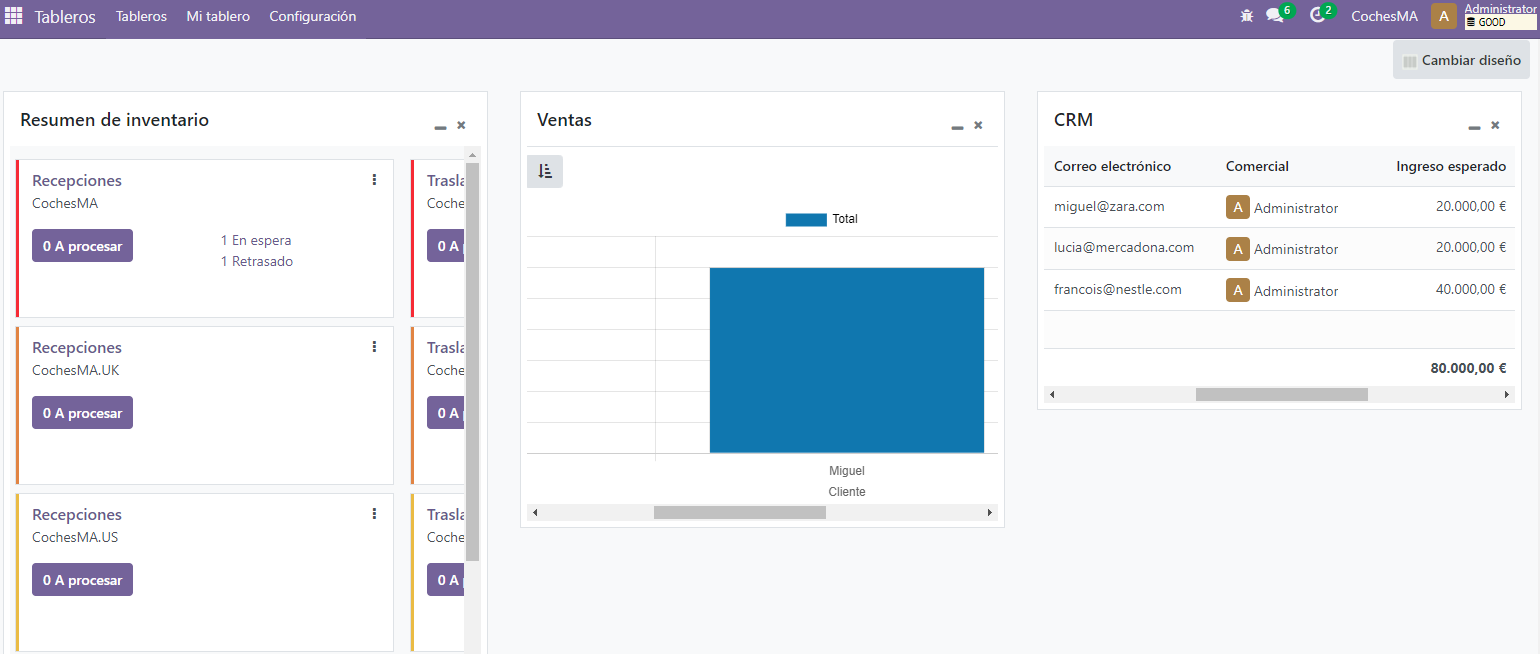
\includegraphics[width=1\linewidth]{fotosDecisiones/admin.png}
    \caption{Tablero del administrador}
    \label{fig:enter-label}
\end{figure}
Además, se ha personalizado los tableros de dos usuarios, Marcus y James. Marcus es gestor de personal por lo que se le ha asignado un informe de los empleados y del reclutamiento de la empresa, porque son los que necesita un gestor de personal para analizar y ejercer sus responsabilidades, tomar decisiones estratégicas relacionadas con la gestión del talento, la contratación y los empleados, facilitando la optimización de los recursos humanos. 
\begin{figure}[h]
    \centering
    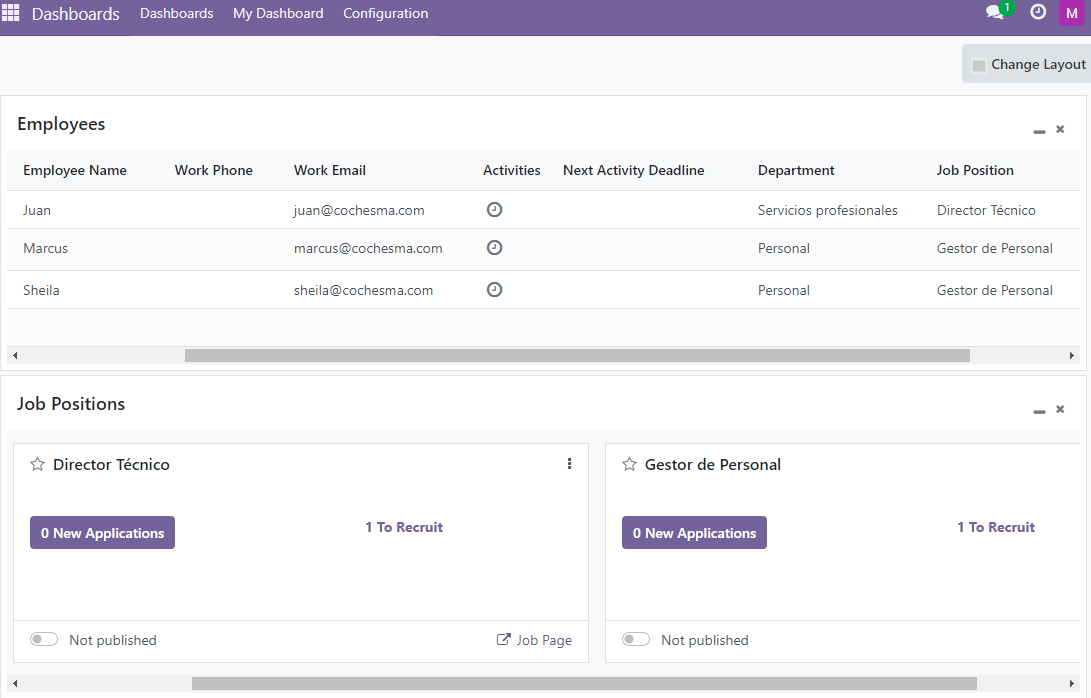
\includegraphics[width=0.9\linewidth]{fotosDecisiones/marcus.png}
    \caption{Tablero del gestor de personal Marcus}
    \label{fig:enter-label}
\end{figure}
Por otro lado, a James se le ha asignado el informe de las ventas, ya que proporciona una visión global del rendimiento de ventas, facilita la identificación de tendencias y contribuye a la optimización de recursos y estrategias de ventas.
\newpage
\begin{figure}[h]
    \centering
    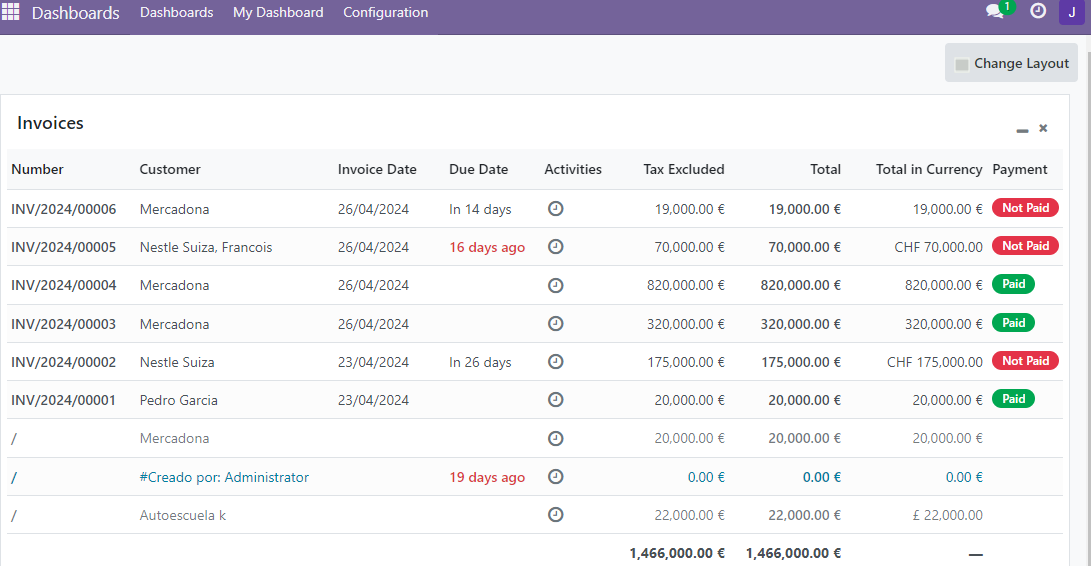
\includegraphics[width=1\linewidth]{fotosDecisiones/james.png}
    \caption{Tablero del gestor de ventas James}
    \label{fig:enter-label}
\end{figure}

Por ultimo, hemos modificado el diagrama BPMN \ref{fab} para representar la interacción entre el módulo de fabricación con este módulo descrito. Este nuevo diagrama es la figura \ref{bi}

\begin{figure}[h]
    \centering
    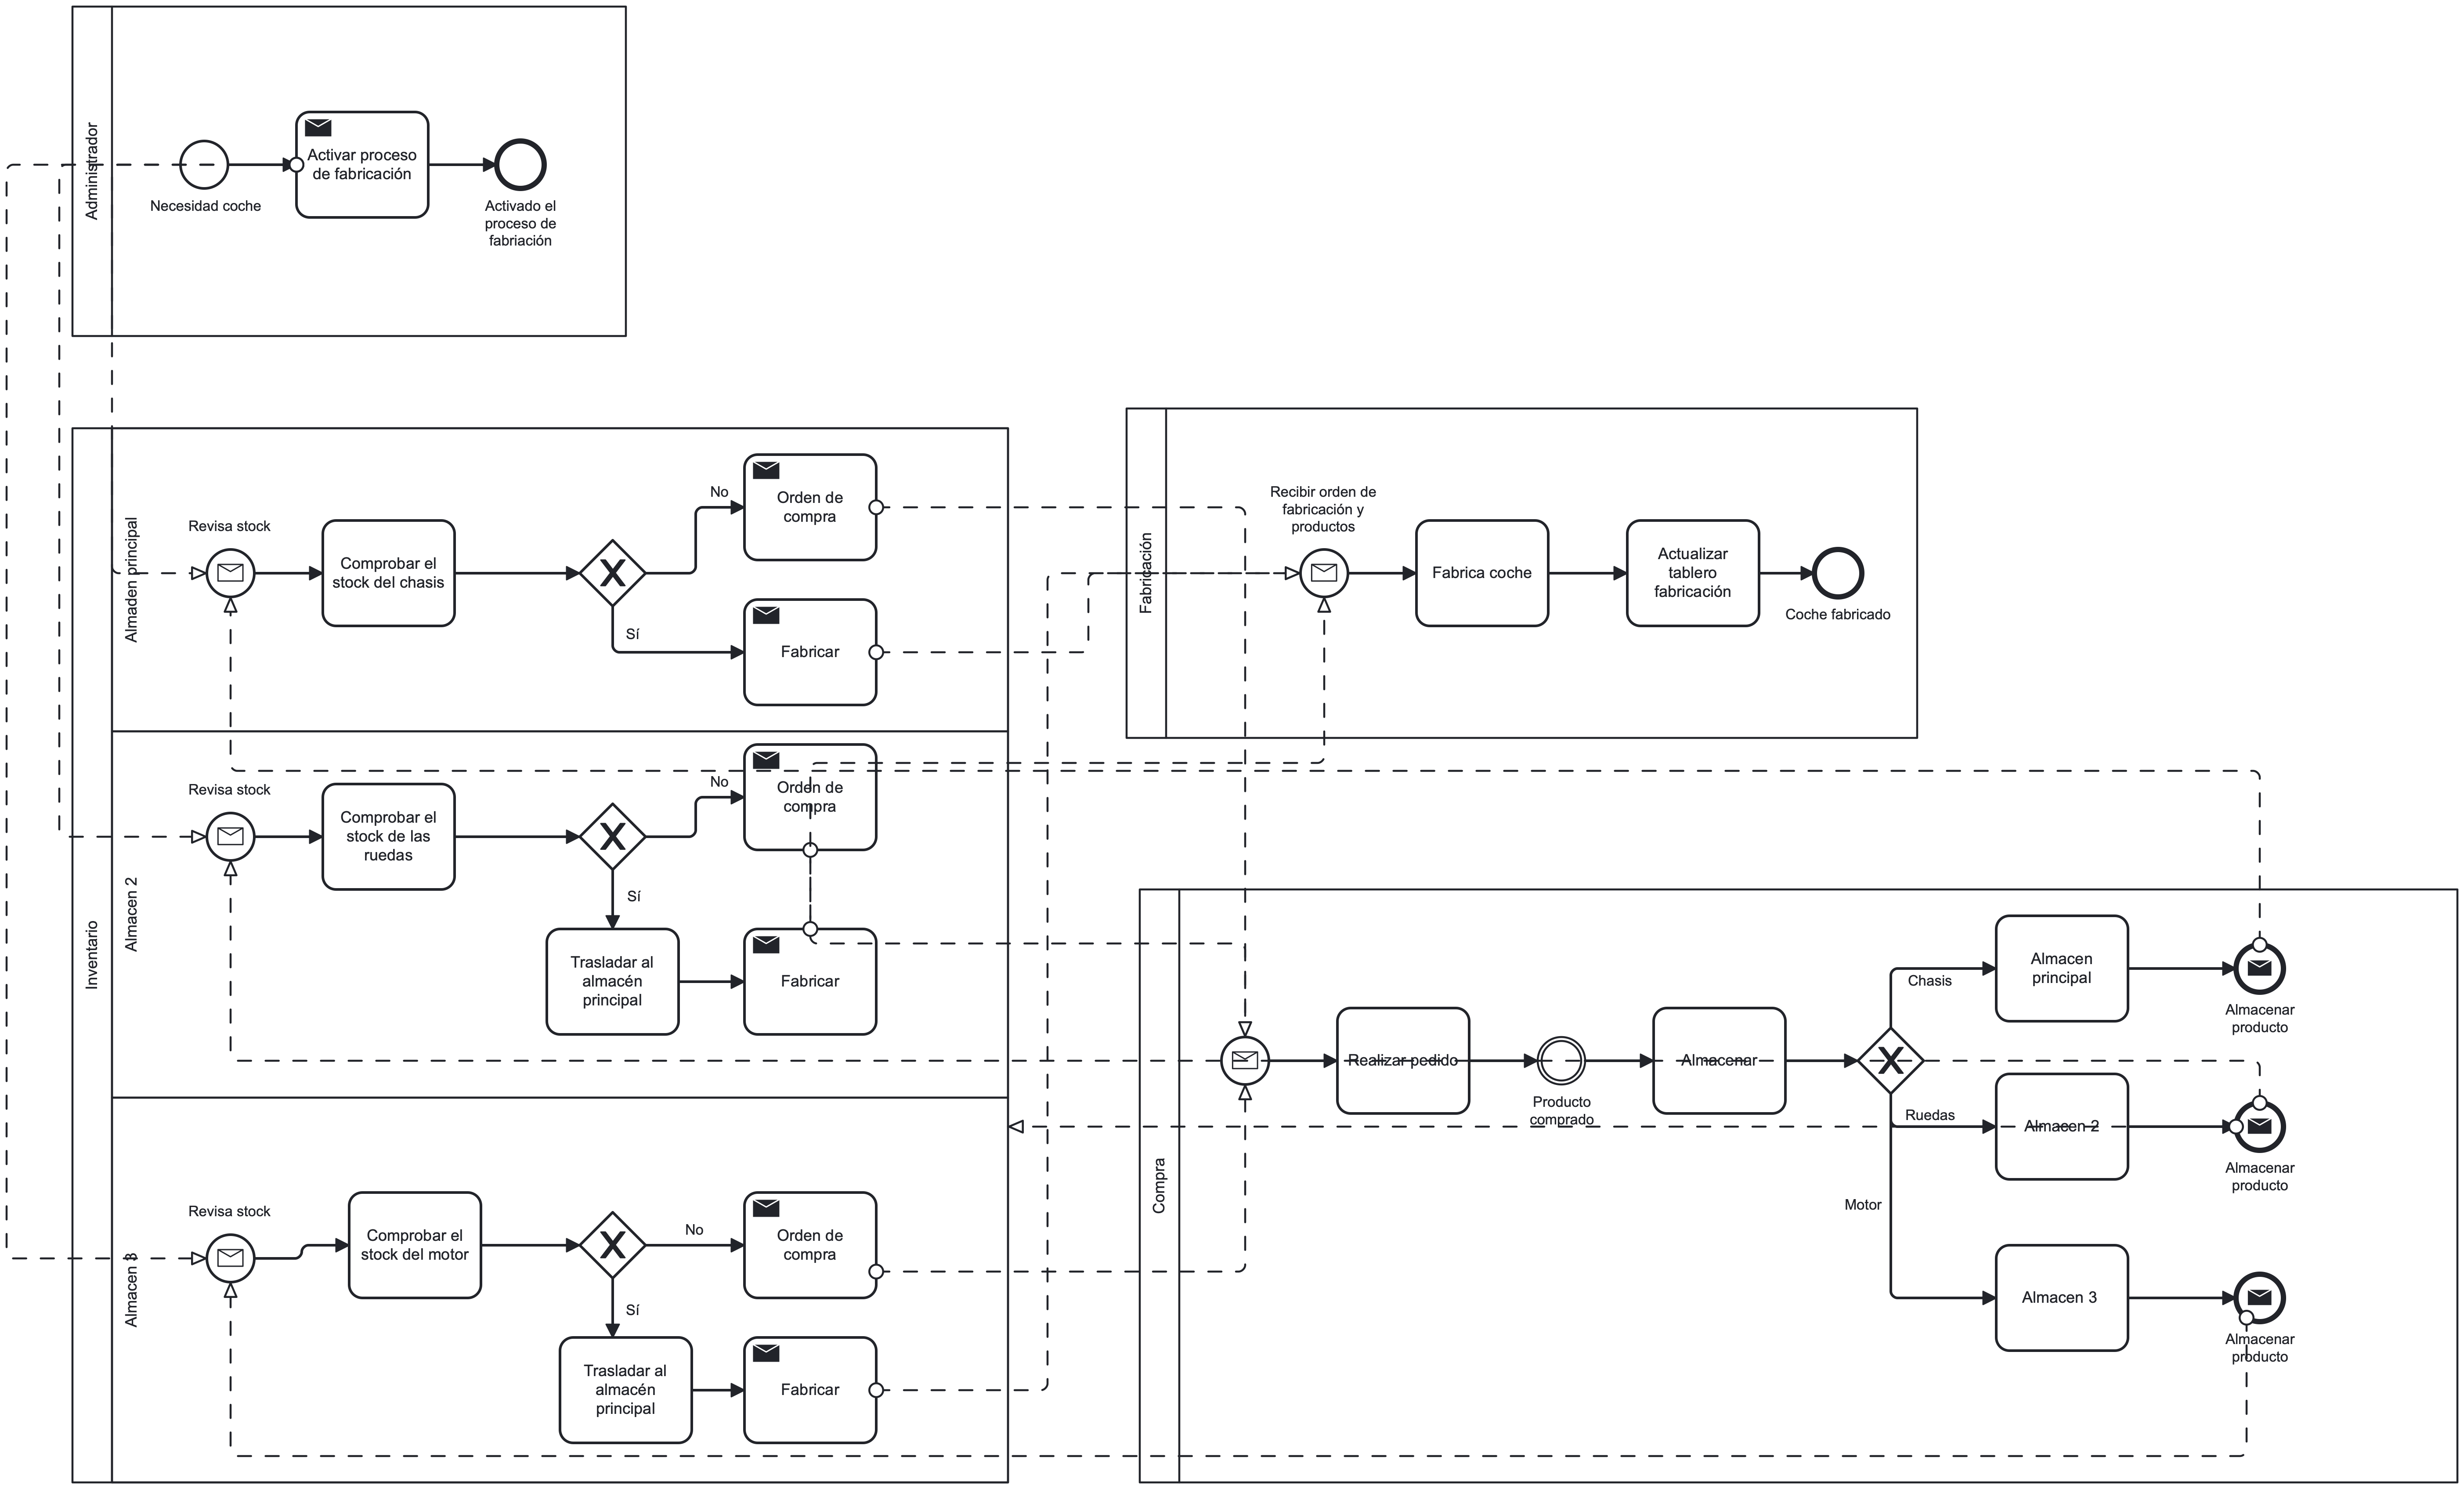
\includegraphics[width=1\linewidth]{fotosGestFab/BI.png}
    \caption{Diagrama BPMN 2.0 modificado, añadiendo la interacción con el tablero de inventario}
    \label{bi}
\end{figure}
\subsection{Conclusiones}
Se ha logrado integrar la funcionalidad de Business Intelligence en Odoo mediante el módulo de Tableros, lo que permite a cada usuario, aprovechar los datos generados para tomar decisiones mediante la creación de dashboards personalizados. Este módulo es fácil de incorporar en Odoo, sin embargo, hay que destacar que si no se han implementado otros módulos que generen los datos necesarios, los tableros pueden perder gran parte de su valor.
\paragraph{}
Por otro lado, el módulo de Tableros proporciona una manera sencilla de personalizar la visualización de datos. No obstante, es importante mencionar que Odoo no ofrece una forma rápida de configurar Tableros, ya que es necesario acceder a cada módulo individualmente para añadir la vista, en lugar de contar con una vista centralizada donde se puedan añadir de manera más eficiente.
